%!TEX root = ../../../thesis.tex

The work throughout the remainder of this thesis is based upon an interface model put forward by my supervisor and a colleague of his, Peter Single.
The model was verified in a single, known concentration of phosphate buffered saline (PBS) at the point I began using it.
Working through the processes taken by my supervisor to create his model, I re-created the model from my own measurements.
By creating a range of solutions of PBS to test against, I fitted parameters of the initial model to the concentration of PBS.
This put me in a good position to compare those solutions to live biological solutions.
That comparison is the main scientific contribution resulting from this work.

\section{The Scott-Single Interface Model}

  \begin{figure}
    \centering
    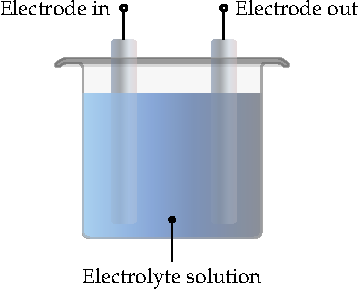
\includegraphics{content/pt2/07-InterfaceModel/graphics/electrode-electrolyte}
    \caption{\label{fig:electrode-electrolyte}Electrodes submerged in an electrolyte solution, such a system can be described by the Scott-Single Interface Model.}
  \end{figure}

  Jonathan Scott and Peter Single recently published an electrical model of an implantable electrode array in saline in 2013 \cite{ScottSingle2013}.
  The intention of that model was to simulate the electrical impedance that a medical implant device would see once implanted into a human spinal cavity.
  It is also general enough to use in any situation where electrodes are placed in an electrolyte solution, such as depicted in \cref{fig:electrode-electrolyte}.

  \begin{figure}
    \centering
    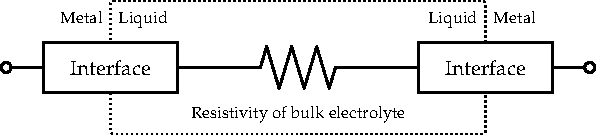
\includegraphics{content/pt2/07-InterfaceModel/graphics/simpleElectrodeElectrolyteModel}
    \caption{\label{fig:pt2-simpleElectrodeElectrolyteModel}Connection diagram of two electrodes (with their interface models) connected together by the resistivity of an electrolyte solution.}
  \end{figure}
  The model comes in two parts, the electrode interface, and the resistivity of the electrolyte's bulk.
  \Cref{fig:pt2-simpleElectrodeElectrolyteModel} shows the general electrical configuration of such an electrode-electrolyte system.
  It shows that there are two interfaces per system, and that the liquid side of those two interfaces are joined electrically by the resistance of the electrolyte's bulk resistivity.
  The metal side of the interfaces is what the rest of the circuit would connect to.
  First, the interface model will be explained.


  \subsection{The interface model}

    \begin{figure}
      \centering
      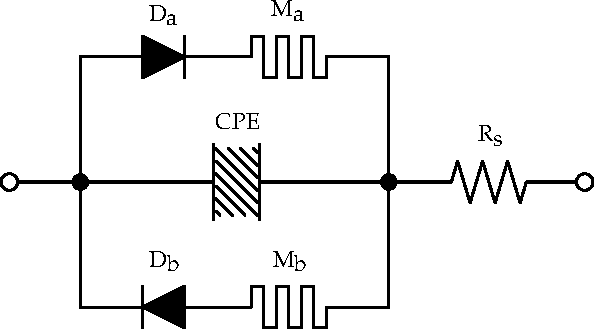
\includegraphics{content/pt2/07-InterfaceModel/graphics/interfaceSchematic}
      \caption{\label{fig:pt2-interfaceSchematic}Electrical schematic of the electrode-electrolyte interface}
    \end{figure}

    The full interface model is represented schematically by \cref{fig:pt2-interfaceSchematic}.
    It represents the transition between the metal of the electrode and the liquid of the electrolyte.
    The model used throughout this thesis is a slightly simplified version of \cref{fig:pt2-interfaceSchematic} in that the memristors have been removed.

    % The Scott-Single interface is modelled by the circuit shown in \cref{fig:pt2-interfaceSchematic}.
    % Each of the components and their functions will be explained in the coming sections.
    % It is important to realise that this model only represents a single interface between metal and electrolyte.
    % By itself it is incapable of simulating any useful electrode/electrolyte system.
    % For that, a minimum of two interfaces must be used - one as a cathode and one as an anode.
    % Additionally, some model of the electrolyte resistivity needs to connect the two interfaces.


    % \Cref{fig:pt2-simpleElectrodeElectrolyteModel} shows the smallest/simplest use of the interface model.
    % This configuration represents two electrodes placed in an electrolyte solution.
    % It allows simulation of impedance between those electrodes and can be connected to other electronic circuits.
    % A model like this is only valid for a two electrode system.
    % Because the electrode array in our application has eight electrodes, the model is more complex.
    % In full, that model will have eight electrode interfaces and a resistor network connecting each interface.

    \subsubsection{Interface series resistance: Resistor}
      The series resistor at the right hand side of the model schematic (labelled $R_{S}$) represents the purely resistive component of the interface's impedance.
      As it is series with all other components in the interface model, there is no way for charge to cross the interface without encountering this resistance.
      The parameter used to denote the interface's series resistance is:
      \begin{itemize}
        \item $R_S$ -- The series resistance of the interface
      \end{itemize}

    \subsubsection{Polar effects: Constant phase element}
      At the centre of the model is the constant phase element, or CPE.
      A CPE, or fractional pole capacitor, is a device that behaves like a cross between a capacitor and a resistor.
      They are primarily used to describe the capacitance of double layer interfaces, the function it serves in this model.
      It is capacitive in the sense that voltage leads current, but by an amount less than \SI{90}{\degree}.
      Mathematically, the \SI{90}{\degree} angle between sinusoidal voltages and currents in a capacitor is a result of the capacitors current being $I(t) = C \times \frac{dV(t)}{dt}$.
      When $V(t)$ is a sine wave, this becomes $I(t) = C \times \frac{d Sin(t)}{dt}$, which is the same as $I(t) = C \times Cos(t)$.
      The angle between Sine and Cosine is always 90, and this is why a capacitors impedance is \SI{-90}{\degree} out of phase.
      A CPE, on the other hand, has a phase angle somewhere \emph{between} 0 and \SI{-90}{\degree}.
      This requires a fractional differentiation of $I(t) = C \times \frac{dV(t)}{dt}$, something uncommon outside of pure mathematics.
      A consequence of having a current/voltage relationship of less than \SI{90}{\degree}, a CPE'S impedance magnitude decays at a rate lower than 20$\frac{dB}{decade}$.

      SPICE, or any other commonly used circuit simulators, does not support fractional pole capacitors so entering one into the model will require building it up from discrete components.
      \begin{figure}[h]
        \centering
        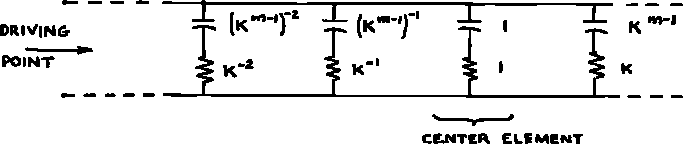
\includegraphics{content/pt2/07-InterfaceModel/graphics/Morrison-RC}
        \caption{\label{graph:pt2-morrisonCPE}Ralph Morrison's implementation of a constant phase element using an infinite array of resistor-capacitor pairs (taken from Morrison's paper -- \cite{Morrison1959}).}
      \end{figure}
      In 1959, Morrison demonstrated a way of creating constant phase elements from an infinite array of resistor-capacitor (RC) pairs \cite{Morrison1959}.
      One of Morrison's implementations of a constant phase element is presented as \cref{graph:pt2-morrisonCPE}.
      Each parallel branch has precisely chosen resistor and capacitor values such that when summed together the impedance magnitude versus frequency is a constant slope, i.e., the impedance does not flatten at a particular frequency as it would with a single RC pair.
      Creating any element comprised of an infinite number of sub-elements is not possible, but by selecting only those elements that contribute to the bandwidth of interest the result is the same within the selected frequency window.
      Using that method and selecting only RC pairs with a cut-off frequency in the range of \SI{1}{\milli\hertz} to \SI{1}{\mega\hertz}, a practical CPE element is created.

      \begin{figure}
        \centering
        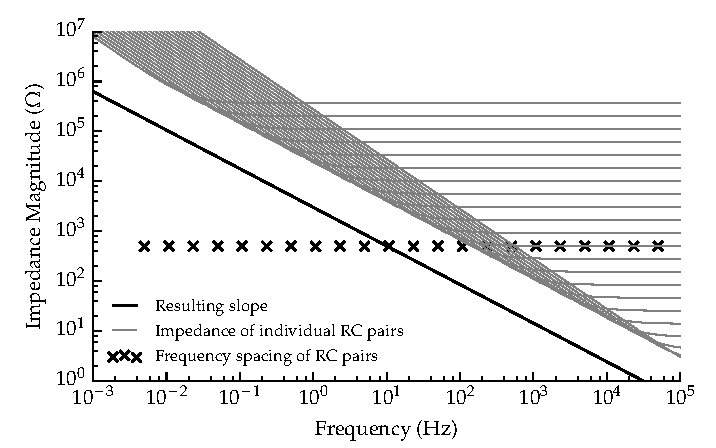
\includegraphics{content/pt2/07-InterfaceModel/graphics/graph_cpe_creation}
        \caption{\label{graph:pt2-cpe_creation}Graph showing how a non \SI{20}{\decibel} per frequency decade}
      \end{figure}

      \Cref{graph:pt2-cpe_creation} shows the individual contributions from each RC branch in an implementation of a CPE.
      Each of grey trace represents a single RC branch in the CPE element, each displaying a high-pass filter slope.
      The value of the resistor in each branch is evident by the vertical spacing of the traces, clearly visible to the right of the graph.
      The branches in this particular example have been spaced in the frequency domain at a density of three per decade, as shown by the black crosses.
      This means that per decade of frequency, there are three corner frequencies, each relating to an RC pair.
      Because each of there branches are in parallel the total response of the CPE is the sum of each branch, that response is shown as the black trace on the graph.
      The critical observation is that the slope of the resulting trace is not the same as each of the individual branches.
      This allows the CPE to behave fractionally as a capacitor, being anywhere between resistive (flat response) and capacitive (\SI{20}{\decibel}/decade slope).

      The CPE is represents readily reversible reactions, polar reorientation, and ionic repulsion and attraction between the electrode surface and electrolyte.
      It is capacitive in nature because each of these mechanisms store charge, which can be drawn back by reversing the applied electromotive force.
      Parameters used to describe the behaviour of the CPE are:
      \begin{itemize}
        \item $m$ -- Slope of the CPE's frequency response
        \item $k$ -- Spacing, or density, of R-C branches with frequency
        \item $|Z|$ @ \SI{1}{\kilo\hertz} -- Sets the vertical position of the magnitude of CPE's frequency response at a known frequency
      \end{itemize}


    \subsubsection{Faradaic reactions: diodes}
      If the voltage placed across the interface is kept within certain limits, the CPE and series resistance ($R_{S}$) would be all that is necessary to accurately mimic a single electrode-electrolyte interface.
      But once the electric potential across the interface becomes high enough, Faradaic reactions will occur at the electrode's surface.
      Faradaic reactions are reactions involving charge transfer, adding ionised species to the electrolyte and often producing gas.
      Gas, or any new species, is bad news in an implanted setting as this causes damage to the patient.
      Possible faradaic reactions between saline and platinum electrodes are:
      \begin{eqnarray}
          Pt + H_{2}O &\Leftrightarrow& PtO + 2 H^{+} + 2 e^{-}\\
          PtO + H_{2}O &\Leftrightarrow& PtO_{2} + 2 H^{+} + 2e^{-}\\
          Pt + H^{+} & \Leftrightarrow & Pt-H\\
          Pt + H_{2}O + e^{-} &\Leftrightarrow& Pt-H+OH^{-}
      \end{eqnarray}

      The electrical current density through an electrode as a function of electrode overpotential and the cathodic and anodic reactions occurring at each electrode is given by:
      \begin{equation}
        i_{net} = i_{0} \left\{ \frac{[O]_{(0,t)}}{[O]_{\infty}}e^{-\alpha_{c}nf\eta} - \frac{[R]_{(0,t)}}{[R]_{\infty}}e^{(1-\alpha_{c})nf\eta}\right\}
        \label{eqn:pt-2_butlerVolmerEquation}
      \end{equation}
      % \Cref{eqn:pt-2_butlerVolmerEquation} describes electrical current density through an electrode as a function of electrode overpotential and the cathodic and anodic reactions occurring at each electrode.
      This is the current-overpotential equation and is derived from the more general Butler-Volmer equation \cite{Merrill2005,ScottSingle2013}.
      In \cref{eqn:pt-2_butlerVolmerEquation}, $i_{net}$ is the net Faradaic current across the electrode/electrolyte interface,
      $i_{0}$ is the exchange current density,
      $[O]_{(0,t)}$ and $[R]_{(0,t)}$ are the concentrations at the electrode surface as a function of time,
      $[O]_{\infty}$ and $[R]_{\infty}$ are concentrations of reactant in the bulk electrolyte,
      $\alpha_{c}$ is the cathodic transfer coefficient (approximately 0.5),
      $n$ is the number of moles of electrons per mole of reactant oxidised,
      $f$ is Faraday's constant divided by the the product of the gas constant and the absolute temperature ($F/RT$),
      and $\eta$ is the electrode overpotential.
      This equation describes the forward and reverse electrical current through an electrode by separating the forward and reverse reactions; oxidisation and reduction.
      \begin{equation}
        I = i_0 e^{V_D / n V_T}
        \label{eqn:pt-2_diodeEquation}
      \end{equation}
      Taking a single half of the equation, either the reduction or oxidisation, yields an equation that is similar to that of a diode; an observation made by McAdams and utilised in the Scott-Single model \cite{McAdams1995}.
      The standard diode equation is shown as \cref{eqn:pt-2_diodeEquation}, where
      $I$ is the current through the diode,
      $i_0$ is the diode saturation current,
      $V_D$ is the potential across the diode,
      $n$ is the diode's ideality factor,
      $V_T$ is the thermal voltage (defined as the product of Boltzmann's constant and temperature divided by the charge on an electron).
      The parameters used to describe the behaviour of the diode are:
      \begin{itemize}
        \item $i_0$ -- the diode's saturation current
        \item $n$ -- the diode's ideality factor
      \end{itemize}
      The diodes themselves can not account for the relative abundance of reactants for the redox reactions, this must be taken care of separately.

    \subsubsection{Species depletion: memristors}

      \begin{figure}[h]
        \centering
        \includegraphics{content/pt2/07-InterfaceModel/graphics/memristorSymbol}
        \caption{\label{fig:pt2-memristorSymbol}Electrical symbol of a memristor, as is used in the original electrode-electrolyte interface model}
      \end{figure}

      A memristor is a two port device that sets its resistance based on its own history.
      Its resistance can either depend on the integral over time of the voltage placed across it or the total charge passed through the device \cite{Kvatinsky2012}.
      Its name is a portmanteau of the word `memory' and `resistor' owing to its use of memory to set its resistance.

      The memristive device models species depletion in the electrolyte by pinching off a diode branch with the amount of current passed through the diode.
      As the specific Faradaic reaction proceeds, it consumes the reactants from the electrolyte bulk until eventually there is none left.
      Increasing the resistance in series with a conducting diode has the effect of removing that diodes current path from the circuit, simulating the depletion of reactants for the modelled reaction.

      Memristors were removed from the model used in this thesis as they added complexity that would yield very little value.
      The diodes are only used to model the \emph{onset} of Faradaic conduction, which is the most relevant parameter of the Faradaic modelling.
      Once these reactions begin, the electrode overpotential has been pushed too far and there is little to be gained from knowing how far the reaction can be run until the reactants have been depleted.
      In an implanted setting it is likely that the electrolyte will circulate throughout the body, bringing new reactants to the electrode's surface over time.
      Species depletion is likely to be a slow process, dependant on the electrolyte volume and species concentration.

      \begin{figure}
        \centering
        \includegraphics{content/pt2/07-InterfaceModel/graphics/interfaceSchematic_noMemristive}
        \caption{\label{fig:pt2-interfaceSchematic_noMemristive}Electrical schematic of the electrode-electrolyte interface without memristors (as used throughout this thesis)}
      \end{figure}

      \Cref{fig:pt2-interfaceSchematic_noMemristive} shows the actual interface model used throughout the remainder of this thesis.
      Although it is slightly different to the Scott-Single interface model, the other parameters are unaffected by the removal of these elements.
      Each of the components of the interface model have now been described.
      A model of the interface on its own is of little value as there will always be two interface models and those models will be separated by the electrolyte itself.


  \subsection{Inter-electrode resistivity}

    Modelling the resistance between two electrodes in a fixed geometry situation is simply a matter of inserting an appropriately sized resistor between the two interfaces.
    The resistance is dependant on the electrolyte's conductivity, the combined surface area of the two electrodes and the distance between them.
    Modelling an electrode array, such as the St. Jude Medical - Octrode, is more complex as it requires a resistor network to describe the inter-electrode resistances.
    An illustration of an Octrode is presented as \cref{fig:StJudeOctrode_Labelled}.

    \begin{figure}
      \centering
      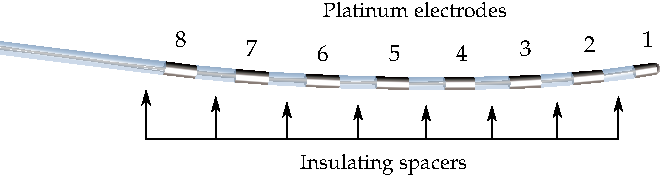
\includegraphics{content/pt2/07-InterfaceModel/graphics/StJudeOctrodeDiagram}
      \caption{\label{fig:StJudeOctrode_Labelled}St. Jude Medical Octrode. An eight electrode array commonly used in spinal stimulation implants. The electrode numbering shown here will be used throughout this work.}
    \end{figure}

    Scott and Single create resistor network for modelling the electrolyte conductivity based on the geometry of the electrodes and the resistivity of the electrolyte.
    By sectioning the surrounding liquid into cylindrical volumes they calculate the equivalent resistance between those volumes both radial and longitudinal directions.
    The radaii of the volumes double at each layer which correspond to a fixed radial resistance between each layer.
    There are two different radial resistances, one for the rings expanding from the insulating spacers, and one for those expanding from the electrode cylinders.
    The two alternate due to each electrode being separated by an insulating spacer.
    The longitudinal resistances quarter in size with each ring layer and after the last radial resistor each node it shorted together.
    The full mesh for the eight electrode array is five layers deep with three rows of padding at each terminating end, totalling two hundred and five resistors in total.
    \Cref{fig:pt2-ResistorMesh} shows the resistor network schematic.
    Further details of how the mesh geometry and resistor values were calculated can be found in \cite{Scott2014}.

    The parameters that describe the resistor mesh are:
    \begin{itemize}
    \item $R_{eri}$ - The initial resistance placed radially from an electrode.
    \item $R_{sri}$ - The initial resistance placed radially from a spacer.
    \item $R_{li}$ - The longitudinal resistance.
    \item Depth - Number of layers between the electrode/spacer and the common end node in the ladder
    \item Padding - Number of spacer layers to be added to the before the first electrode and after the last electrode in the network.
    \end{itemize}

    \begin{figure}
      \centering
      \includegraphics{content/pt2/07-InterfaceModel/graphics/resistorMesh}
      \caption{\label{fig:pt2-ResistorMesh}Resistor mesh used to model the electrical resistance between interface pairs. $R_{li}$ is longitudinal resistance, $R_{sri}$ and $R_{eri}$ is the radial resistance for the spacers and electrodes respectively, and $I$ is an interface.}
    \end{figure}

\section{Electrolyte: Phosphate Buffered Saline}
  The model has been fitted to phosphate buffered saline (PBS) because it is was closest representation of human spinal fluid known at the time.
  Engineers at Saluda used a concentration one-tenth that of a standard solution of PBS as a test solution for their spinal implants as they believed it to be a good match.
  I was not understood how well the one-tenth concentration matched spinal fluid electrically, which is one of the first research questions I set out to answer.
  The ingredients used to make the stock standard PBS concentration solution are given in \cref{tab:pt2-PBS-recipe} and the procedure for creating the full strength stock are as follows.
  \begin{enumerate}
    \item Weigh out day ingredients and combine in stock bottle.
    \item \SI{800}{\milli\litre} of distilled water is added to bottle and solution is stirred until all solids have dissolved.
    \item pH is measured and adjusted to 7.4 by addition of HCL.
    \item The stock solution was mixed up to the target volume of \SI{1000}{\milli\litre}.
  \end{enumerate}

  \begin{table}
    \centering
    \begin{tabular}{r | r | c}
      Ingredient & Quantity & Unit \\
      \hline
      H$_2$O & 1000 & ml \\
      NaCl & 8.00  & g  \\
      KCl  & 0.20  & g  \\
      Na$_2$HPO$_4$ & 1.44 & g \\
      KH$_2$PO$_4$  & 0.24 & g \\
    \end{tabular}
    \caption{\label{tab:pt2-PBS-recipe}Ingredients used to produce one litre of stock solution of phosphate buffered saline.}
  \end{table}

  \begin{table}
    \centering
    \begin{tabular}{r | r | c}
      Stock (ml) & Water (ml) & Final Concentration \\
      \hline
      700.0 &   0.0 & 1.00X \\
      350.0 & 350.0 & 0.50X \\
      175.0 & 525.0 & 0.25X \\
       70.0 & 630.0 & 0.10X \\
       35.0 & 665.0 & 0.05X \\
       17.5 & 682.5 & 0.025X\\
    \end{tabular}
    \caption{\label{tab:pt2-PBS-concentration}Final dilutions of stock to create six \SI{700}{\milli\litre} solutions ranging from 0.025X to 1X standard PBS concentration.}
  \end{table}

  Six bottles of ranging in concentration from full strength (1.0X) to one-fortieth (0.025X) were then made from the stock solution.
  \Cref{tab:pt2-PBS-concentration} shows the volumetric dilution used to create the six concentrations of PBS that are then used to fit the model parameters to.


\section{Methods Of Parameter Extraction}
  The model has a number of parameters that are used to set the behaviour of each of the components.
  Finding suitable values for each of the parameters is critical in ensuring that the final model offers a good representation of the electrode-electrolyte system.
  The trick to finding suitable parameter values lies in selecting useful measurements of each part of the model, usually by isolating the measurement as much as possible from other model elements.
  The following sections describe the measurements used to determine parameters used in the final model.
  Ideally each element in the model would be measured separately, but in some cases it is not possible to totally isolate two areas.
  Scott and Single found a set of parameters that described the Octrode in a one-tenth concentration solution of phosphate buffered saline (PBS).
  In this section I create six different solutions of PBS ranging in concentration from 1.0x to 0.025x the concentration of a standard PBS solution.
  I extend the Scott-Single model to work over a range of concentrations of PBS by adding another parameter to the model - PBS concentration.


  \subsection{Resistivity}
    In order to find the parameters of any elements within the electrode-electrolyte interface it is first necessary to find the inter-electrode resistances.
    This is because elements of the model can not be measured in isolation since the resistivity of the electrolyte solution will always present itself between a measurement apparatus and the element of interest.
    I start by determining the resistances used in the resistor mesh using the same method as was used by Scott and Single \cite{Scott2014}.
    Once those resistances are accounted for, the behaviour of components in the interface can be calculated from measurements that included those inter-electrode resistances by subtraction.

    \begin{figure}
      \centering
      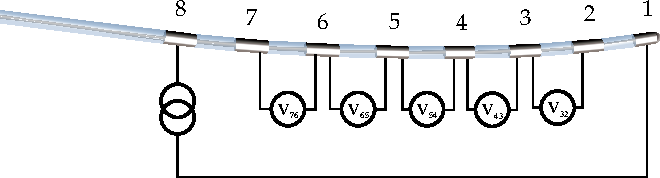
\includegraphics{content/pt2/07-InterfaceModel/graphics/TransimpedanceMeasurements_Stim81}
      \caption{\label{fig:pt2-transimpedanceMeasurementDiagram_81Stim}Measurement schematic of trans-impedance measurements where electrodes eight and one are driven and the remainder are used in voltage differential measurements.}
    \end{figure}

    \begin{figure}
      \centering
      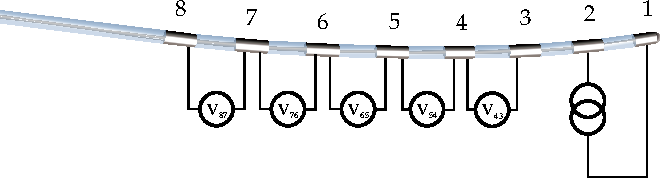
\includegraphics{content/pt2/07-InterfaceModel/graphics/TransimpedanceMeasurements_Stim21}
      \caption{\label{fig:pt2-transimpedanceMeasurementDiagram_21Stim}Measurement schematic of trans-impedance measurements where electrodes two and one are driven and the remainder are used in voltage differential measurements.}
    \end{figure}

    Scott and Single measure trans-impedance between pairs of electrodes in two different configurations where a defined AC current is driven between a pair of electrodes.
    Data from these measurements is tabulated so each row contains the AC current forced between the two stimulus electrodes and a voltage measured between a pair of non-driven electrodes.
    By measuring the voltage across pairs of non-driven electrodes using a suitably high impedance measurement, those measurements will correspond to the voltage difference in the electrolyte.
    For this method to work it is assumed that the current passing through each non-driven interface is zero, and therefore no voltage is dropped between the electrode's metal and the electrolyte solution at the electrode's surface.
    This means that voltage differentials can only be measured on the non-driven electrodes.
    \Cref{fig:pt2-transimpedanceMeasurementDiagram_81Stim,fig:pt2-transimpedanceMeasurementDiagram_21Stim} show the two measurement configurations used to collect transimpedance data.
    Those transimpedance results are recreated using a simulated mesh of resistors with fitted values to the three resistor parameters.
    An optimisation routine can be used to find the three values that create a mesh that matches the measured values as close as possible, as summarised in \cref{tab:pt2-parameterDesc-ResistorMesh}.

    \begin{table}
      \begin{center}
        \begin{tabular} {r | l}
          Parameter & Determined from:\\
          \hline
          $R_{eri}$ & optimised fit via SPICE simulation\\
          $R_{sri}$ & optimised fit via SPICE simulation\\
          $R_{li}$ & optimised fit via SPICE simulation\\
          Padding & previous value of 3 rows used (from Scott \& Single)\\
          Depth & previous value of 5 layers used (from Scott \& Single)
        \end{tabular}
      \end{center}
      \caption{\label{tab:pt2-parameterDesc-ResistorMesh}Parameters determined by an optimised fit between a simulated mesh and transimpedance measurements.}
    \end{table}


  \subsection{Constant phase element and series resistance}
    \begin{figure}[h]
      \centering
      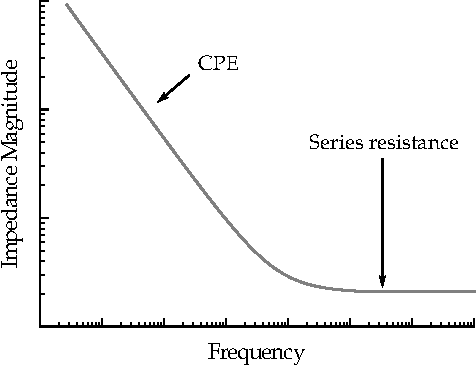
\includegraphics{content/pt2/07-InterfaceModel/graphics/graph_cpePlotGeneral}
      \caption{\label{fig:pt2-graph_cpePlotGeneral}Log-log plot of frequency vs impedance magnitude of a single interface and inter-electrode impedance. The response of the CPE and that of the total series resistance is separated in the frequency domain.}
    \end{figure}
    By accounting for the value of resistance seen between electrodes it is now possible to probe deeper into the interface model.
    Calculation of both the CPE and the series resistance ($R_S$) is made via impedance spectroscopy.
    It is possible to use the applied frequency to separate the response of the CPE from that of the series resistance of a single interface and inter-electrode resistance.
    The impedance of the CPE dominates below \SI{10}{\hertz}, where its slope and magnitude can be determined.
    At higher frequencies, greater than \SI{1}{\kilo\hertz}, the series resistance of both the interface ($R_S$) and the previously determined inter-electrode resistance is evident.
    This separation of responses is illustrated in \cref{fig:pt2-graph_cpePlotGeneral}.
    Subtracting the inter-electrode resistance (determined previously) from the resistive element yields just the interface's series resistance ($R_S$).
    Parameters for the CPE, such as slope and vertical position, are then read off the low frequency part of the trace where the slope is not disturbed by the resistive part.
    These parameters are summarised in \cref{tab:pt2-parameterDesc-CPE}.

    \begin{table}
      \begin{center}
        \begin{tabular} {r | l}
          Parameter & Determined from:\\
          \hline
          $k$ & previous value of 3 branches used (from Scott \& Single)\\
          $m$ & slope of |Z| vs. frequency response\\
          |Z| @ \SI{1}{\hertz} & impedance magnitude at \SI{1}{\hertz}\\
          $R_S$ & impedance at high frequency (\SI{10}{\kilo\hertz}) end of the trace
        \end{tabular}
      \end{center}
      \caption{\label{tab:pt2-parameterDesc-CPE}Parameters determined from impedance spectroscopy measurements of electrode-electrolyte interface.}
    \end{table}


  \subsection{Faradaic currents}
    Measurement of Faradaic current requires pushing the electrode overpotential until reactions at the electrode's surface begin.
    Electrical currents involved with Faradaic conduction increase exponentially with increasing electrode overpotential.
    Scott and Single used a triangular voltage stimulus to identify the onset of Faradaic conduction at the interface.
    The triangular wave is equivalent to a constant ramp-up and ramp-down of voltage placed across the interface.
    It was mentioned earlier that current flowing into a capacitor is given by: $I(t) = C \times \frac{dV(t)}{dt}$.
    When $\frac{dV(t)}{dt}$ is a constant, as is the case for any constant ramp-up or ramp-down voltage stimulus, the current becomes a constant.
    It is assumed that the fractional differentiation of the current equation will still yield a relatively constant current in light of the capacitor being a CPE.
    By slowly ramping the electrode overpotential up the current should be constant up to a point where it becomes exponential.
    The voltage corresponding to the point at which the current draw becomes exponential will be used to determine the onset of Faradaic conduction.
    That point, together with the rate of growth, would then used to fit values for $i_0$ and $n$, the diode's saturation current and ideality factor respectively, as summarised in \cref{tab:pt2-parameterDesc-Diode}.
    Problems arose with those measurements, which will be discussed in the following section, that show the behaviour of the CPE was less predictable than expected.


    \begin{table}
      \begin{center}
        \begin{tabular} {r | l}
          Parameter & Description \\
          \hline
          $i_0$ & optimised fit of threshold voltage to measured curve\\
          $n$ & optimised fit of growth rate to measured curve
        \end{tabular}
      \end{center}
      \caption{\label{tab:pt2-parameterDesc-Diode}Parameters determined from fitting diode parameters to measured response of Faradaic current.}
    \end{table}
